%!TEX root = origin.TEX
\chapter{Resultados de la tesis}
\pagenumbering{arabic}
\setcounter{page}{127}
\renewcommand{\baselinestretch}{1.2} %doble espacio paratodo el texto
	
	Al culminar con la investigación, para la prueba de resultados de clasificación se dispone de una matriz de confusión. La matriz de confusión es una matriz cuadrada cuyo orden es el número de clases. En las  columnas se presentan las clases reales mientras que en las filas se presentan las clases asignadas por el clasificador, por ende, la suma vertical muestra la distribución real de las clases, mientras que la suma horizontal muestra la distribución de las clases producida por el clasificador.

	El análisis de los clasificadores se hace con base en la matriz de confusión de la cual se obtienen los 4 de los 6 indicadores de desempeño mencionados en la \textbf{Seccion 2.5.3 Indicadores}.

	\begin{itemize}

	\item Prop. de Verdaderos Positivos(Efectividad): {$PVP= \frac{Verdaderos\,Positivos}{{Verdaderos\,Positivos} + {Falsos\,Negativos}}$}
	\item Prop. de Verdaderos Negativos(Especificidad): {$PVN= \frac{Verdaderos\,Negativos}{{Verdaderos\,Negativos} + {Falsos\,Positivos}}$}
	\item Valor Predictivo Positivo (Precisión): {$PPV = \frac{Verdaderos\,Positivos}{{Verdaderos\,Positivos}+{Falsos\,Positivos}}$}
	\item Acuracia (Exactitud): {$ACC= \frac{Verdaderos\,Positivos+Verdaderos\,Negativos}{Total\,de\,Imagenes}$}
	\end{itemize}	
	Donde:
	\begin{itemize}
		\item[--] \textit{Verdaderos Positivos}: Imágenes correctamente indentificadas.
		\item[--] \textit{Falsos Positivos}: Imágenes incorrectamente identificadas.
		\item[--] \textit{Verdaderos Negativo}: Imágenes correctamente rechazadas.
		\item[--] \textit{Falsos Negativos}: Imágenes incorrectamente rechazadas.
	\end{itemize}
	
	Utilizando los anteriores indicadores, podemos obtener dos más:
	\begin{itemize}
		\item Curvas ROC : Relación entre Efectividad y Especificidad
		\item Curvas PR  : Relación entre Precisión y Efectividad(Recall)
	\end{itemize}

	
	Las curvas ROC (Característica Operativa del Receptor, del inglés - \textit{Receiver Operating Characteristic}) define un sistema de coordenadas usadas para visualizar el desempeño del clasificador. Las curvas ROC presentan el compromiso entre efectividad (sensibilidad) y especificidad del clasificador, un aumento en la sensibilidad está acompañado por un decremento en la especificidad. Esto significa que la esquina superior izquierda de la gráfica es el punto ideal, debido a que muestran la relación entre las muestras clasificadas adecuadamente (\textit{Proporción de Verdaderos Positivos} - PVP) y las muestras que no pertenecen a la clase pero se clasificaron como si lo fueran (\textit{Proporción de Falsos Positivos - PFP}). Esta última, calculada a través de la Especificidad (PVN), siendo:
	\begin{center}
	{$PFP= 1 - PVN$}
	\end{center}

	Las curvas ROC se utilizan normalmente en la clasificación binaria para estudiar la salida de un clasificador. Para dibujarlas se construye la línea convexa formada por los puntos (PFP, PVP) de los clasificadores que se estén evaluando, junto con los puntos de los clasificadores triviales (0,0) y (1,1). La curva más cercana a los bordes izquierdo y superior en el espacio ROC, es la prueba más acertada porque significa que hay mayor acierto. La curva que más se acerque a la diagonal de 45 grados en el espacio ROC, es la prueba menos acertada. Para extender la curva ROC y obtener una área ROC a la clasificación de múltiples clases, como es el caso de esta investigación, solo es necesario binarizar la salida. Se puede dibujar una curva ROC por clase, pero también se puede dibujar una curva ROC considerando cada elemento de la matriz de confusión por clase, como una predicción binaria (micro-promedio). Otra medida de evaluación para la clasificación de múltiples clases es el macro promedio, que otorga igual peso a la clasificación de cada etiqueta. El mejor sistema de entrenamiento es el que produce un conjunto de clasificadores que maximice el área bajo la curva (AUC - \textit{Area Under the Curve})\citep{SandovalCereza}.


	De manera similar, las Curvas PR(\textit{Precision -Recall}) represetan la relación entre la Efectividad y Precisión del clasificador. El objetivo es tener un modelo que se posicione en la esquina superior derecha, que básicamente consiste en obtener solo los positivos verdaderos sin falsos positivos ni falsos negativos: un clasificador perfecto. En la situación en la que se tiene clases con cantidades no balanceadas, como es el caso del Dataset- Perú, a menudo es más útil utilizar el Área bajo la Curva PR como indicador del clasificador, \citep{Davis-2006-RPR-1143844-1143874}.


		
	%\newpage
	\section{Señales de Tránsito de Alemania}
		Luego de evaluar cada uno de los 5 modelos durante 100 épocas, el diseño del \underline{\bf modelo E} es el que presentó los mejores resultados.

		\subsection{Tabla de Resultados}


		\begin{table}[H]
			\begin{center}
			\caption{\small{Indicadores de los 5 modelos entrenados en el Dataset - Alemania}}
			\vspace{1.1em}
			\begin{tabular}{|c|c|c|c|c|c|}
			\cline{1-6}
			\textbf{Indicadores}    & \textbf{Modelo A(\%)} & \textbf{Modelo B(\%)} & \textbf{Modelo C(\%)} &\textbf{ Modelo D(\%)} & \textbf{Modelo E(\%)} \\ \hline
			\multicolumn{1}{|c|}{\textbf{PVP}}        & 96.14     & 98.35       & 98.08       & 98.37       & 98.61       \\ \hline
			\multicolumn{1}{|c|}{\textbf{PVN}}        & 99.93     & 99.96       & 99.96       & 99.96       & 99.97       \\ \hline
			\multicolumn{1}{|c|}{\textbf{PPV}}        & 95.69     & 97.52       & 97.57       & 97.78       & 98.01      \\ \hline
			\multicolumn{1}{|c|}{\textbf{AUC-PR}}     & 94.31     & 96.88       & 96.60       & 96.93       & 97.30       \\ \hline
			\multicolumn{1}{|c|}{\textbf{AUC-ROC}}    & 98.04     & 99.15       & 99.02       & 99.17       & 99.29       \\ \hline
			\multicolumn{1}{|c|}{\textbf{ACC}}        & 97.08     & 98.41       & 98.27       & 98.43       & 98.62       \\ \hline
			\end{tabular}
			\end{center}
		\end{table}
		%------------------------------------------------------------------------------------------------------------------------------------------------------------

	 	\subsection{Matriz de Confusión}  
			\begin{figure}[H]
				\begin{center}
				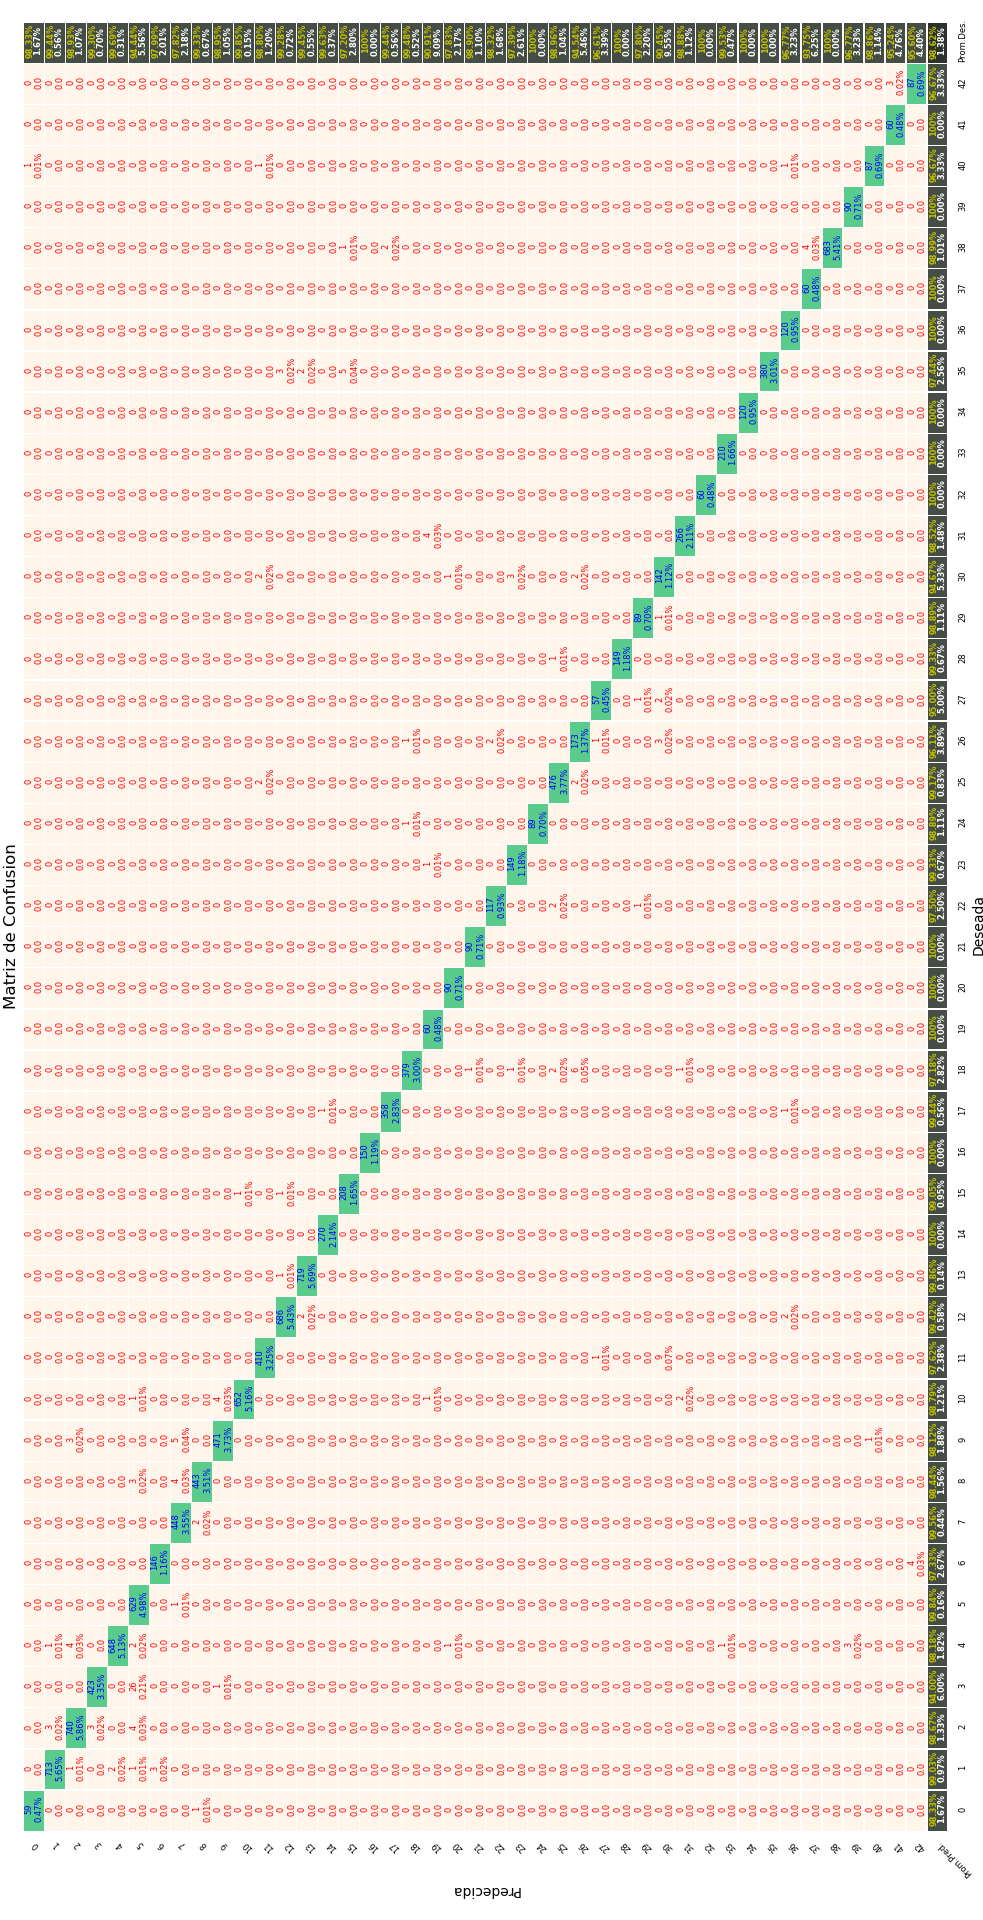
\includegraphics[width=1\textwidth, height=18cm]{images/desarrollo/testResults/german/model_A_A} 
				\end{center}
				\begin{center}
				\caption{\small{Matriz de Confusión del Modelo E - Dataset de imágenes de Alemania}}
				{\small{\fontsize{10}{16.8}\selectfont {Fuente: Elaboración propia}}}
				\end{center}
				\vspace{-1.5em}
			\end{figure}
		%------------------------------------------------------------------------------------------------------------------------------------------------------------
		\subsection{Curvas ROC - AUC}  
					\begin{figure}[H]
						%\begin{center}
						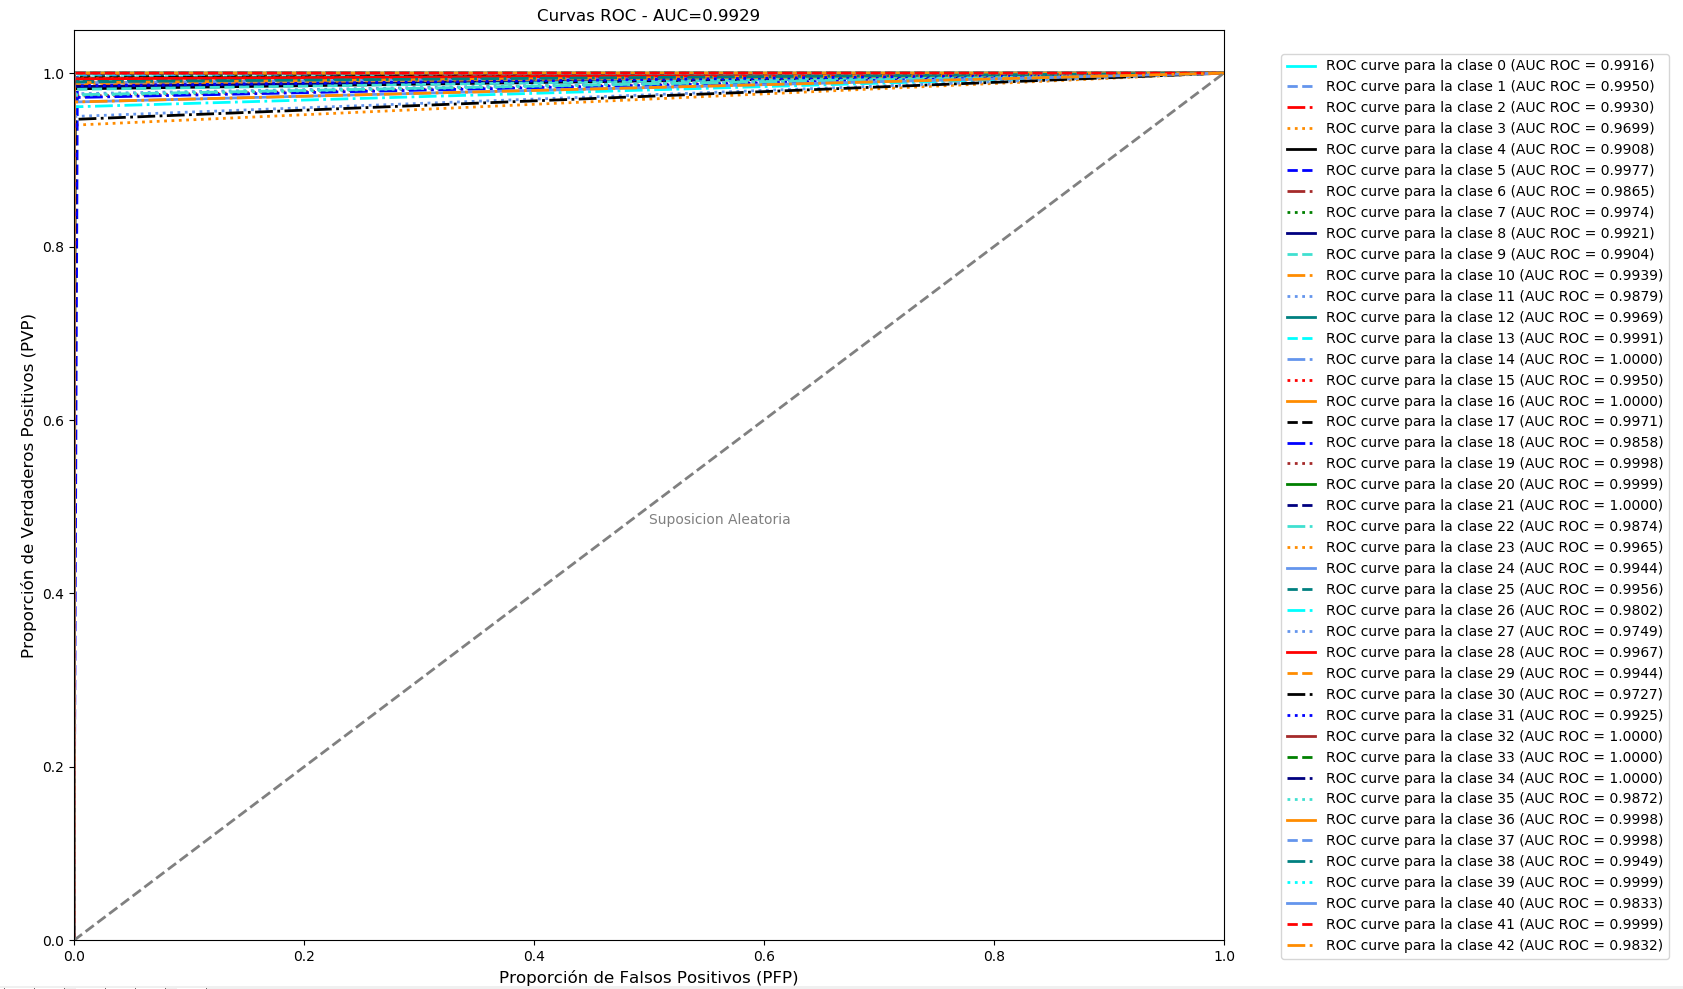
\includegraphics[width=\textwidth, height=7.5cm]{images/desarrollo/testResults/german/ROC_curve_modelE} 
						%\end{center}
						\begin{center}
						\caption{\small{Área debajo de la Curva ROC del Modelo E - Dataset de imágenes de Alemania}}
						{\small{\fontsize{10}{16.8}\selectfont {Fuente: Elaboración propia}}}
						\end{center}
						\vspace{-1.5em}
					\end{figure}
		%------------------------------------------------------------------------------------------------------------------------------------------------------------
		\subsection{Curvas PR - AUC}  
					\begin{figure}[H]
						%\begin{center}
						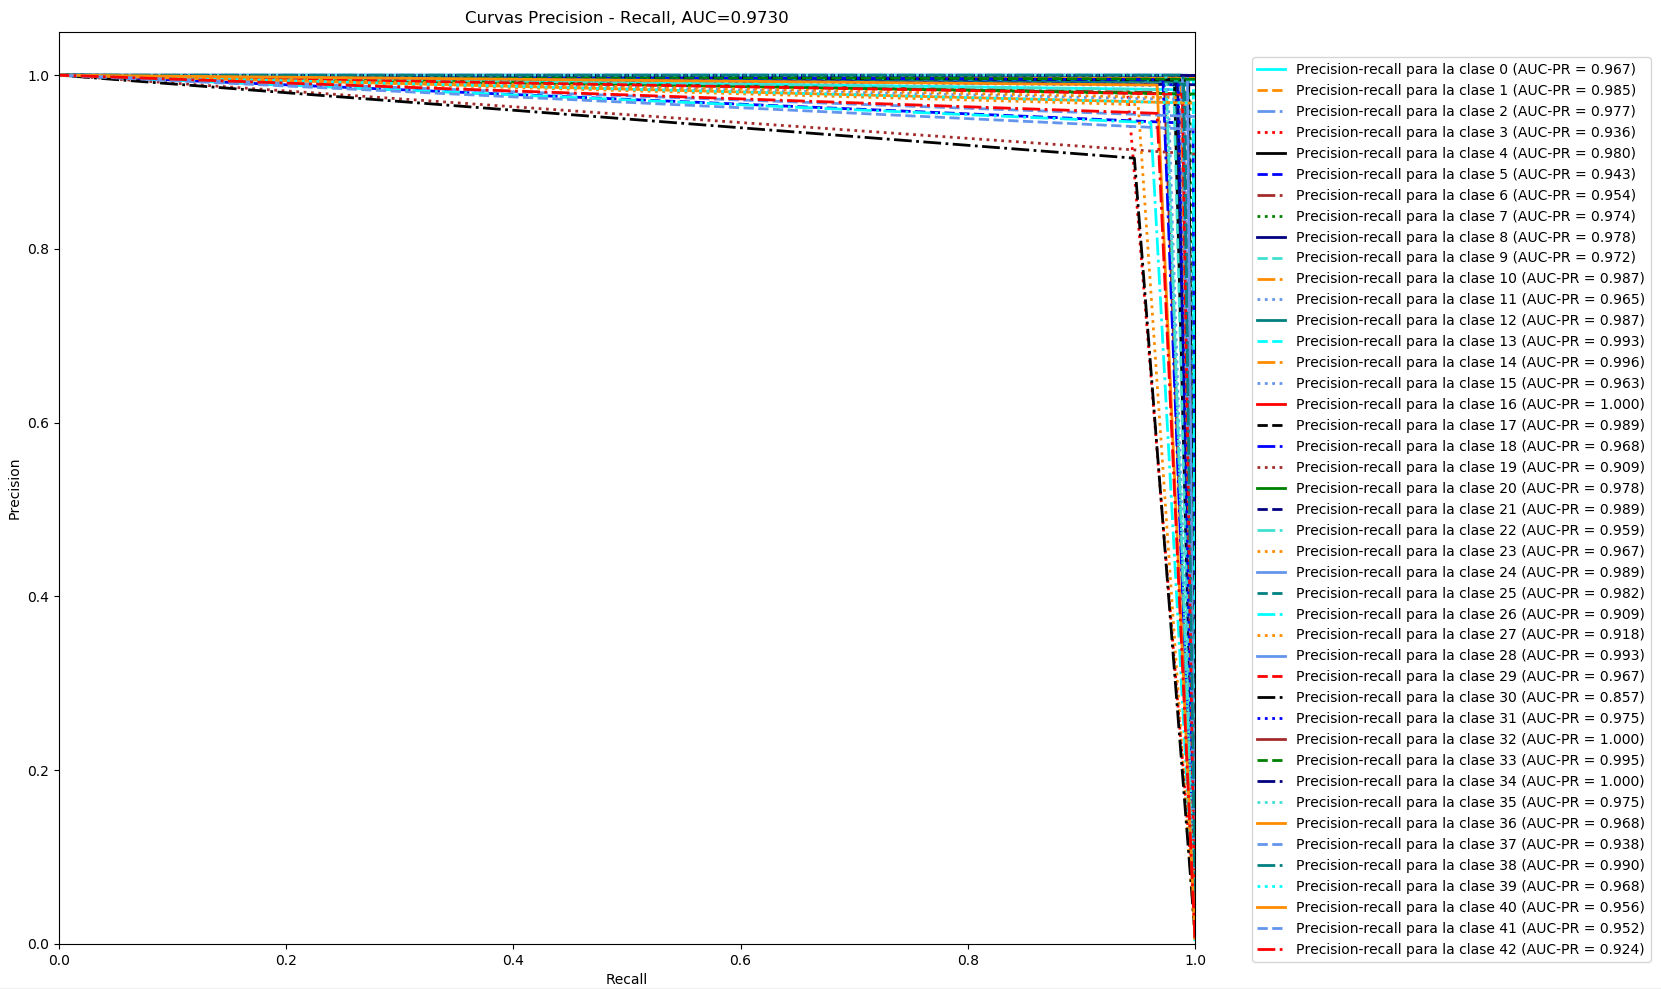
\includegraphics[width=\textwidth, height=7.5cm]{images/desarrollo/testResults/german/PR_curve_modelE} 
						%\end{center}
						\begin{center}
						\caption{\small{Área debajo de la Curva PR del Modelo E - Dataset de imágenes de Alemania}}
						{\small{\fontsize{10}{16.8}\selectfont {Fuente: Elaboración propia}}}
						\end{center}
						\vspace{-1.5em}
					\end{figure}		
	%------------------------------------------------------------------------------------------------------------------------------------------------------------
	
	\section{Señales de Tránsito de Perú}

		Luego de evaluar cada uno de los 5 modelos, el diseño del \underline{\bf modelo E} también es el que presentó los mejores resultados.

		\subsection{Tabla de Resultados}

		\begin{table}[H]
			\begin{center}
			\caption{\small{Indicadores de los 5 modelos entrenados en el Dataset - Perú}}
			\vspace{1.1em}
			\begin{tabular}{|c|c|c|c|c|c|}
			\cline{1-6}
			 \textbf{Indicadores}    & \textbf{Modelo A(\%)} & \textbf{Modelo B(\%)} & \textbf{Modelo C(\%)} &\textbf{ Modelo D(\%)} & \textbf{Modelo E(\%)} \\ \hline
			\multicolumn{1}{|c|}{\textbf{PVP}}        & 95.78     & 99.16       & 99.26       & 98.97       & 99.83       \\ \hline
			\multicolumn{1}{|c|}{\textbf{PVN}}        & 99.44     & 99.91       & 99.92       & 99.86       & 99.97       \\ \hline
			\multicolumn{1}{|c|}{\textbf{PPV}}        & 96.75     & 99.40       & 99.49       & 99.31       & 99.86       \\ \hline
			\multicolumn{1}{|c|}{\textbf{AUC-PR}}     & 94.06     & 98.98       & 99.09       & 98.54       & 99.68       \\ \hline
			\multicolumn{1}{|c|}{\textbf{AUC-ROC}}    & 97.62     & 99.51       & 99.60       & 99.42       & 99.90       \\ \hline
			\multicolumn{1}{|c|}{\textbf{ACC}}        & 96.74     & 99.45       & 99.51       & 98.21       & 99.83       \\ \hline
			\end{tabular}
			\end{center}
		\end{table}
		%------------------------------------------------------------------------------------------------------------------------------------------------------------
	 	\subsection{Matriz de Confusión}  
			\begin{figure}[H]
				\begin{center}
				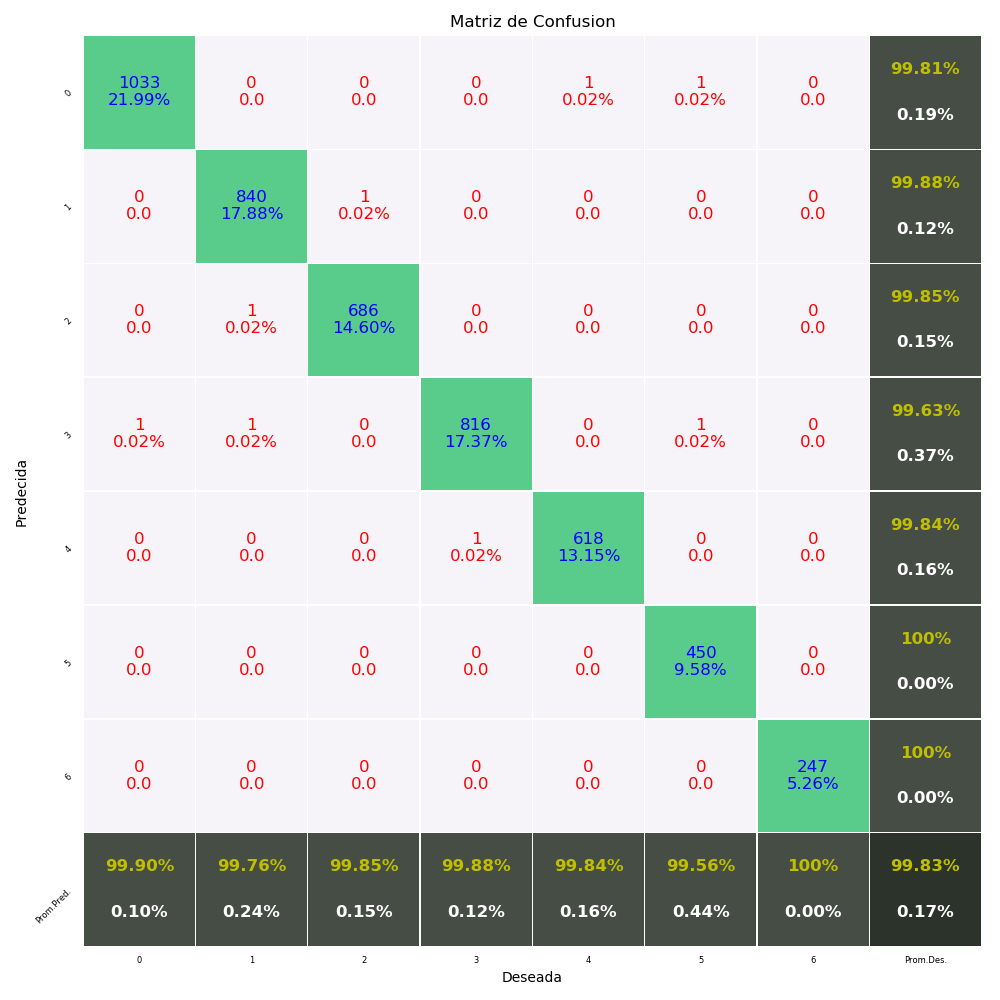
\includegraphics[width=1\textwidth, height=11.2cm,keepaspectratio]{images/desarrollo/testResults/peru/modelE} 
				\end{center}
				\begin{center}
				\caption{\small{Matriz de Confusión del Modelo E - Dataset de imágenes de Perú}}
				
				{\small{\fontsize{10}{16.8}\selectfont {Fuente: Elaboración propia}}}
				\end{center}
				\vspace{-1.5em}
			\end{figure}
		%------------------------------------------------------------------------------------------------------------------------------------------------------------
		\subsection{Curvas ROC - AUC}  
					\begin{figure}[H]
						%\begin{center}
						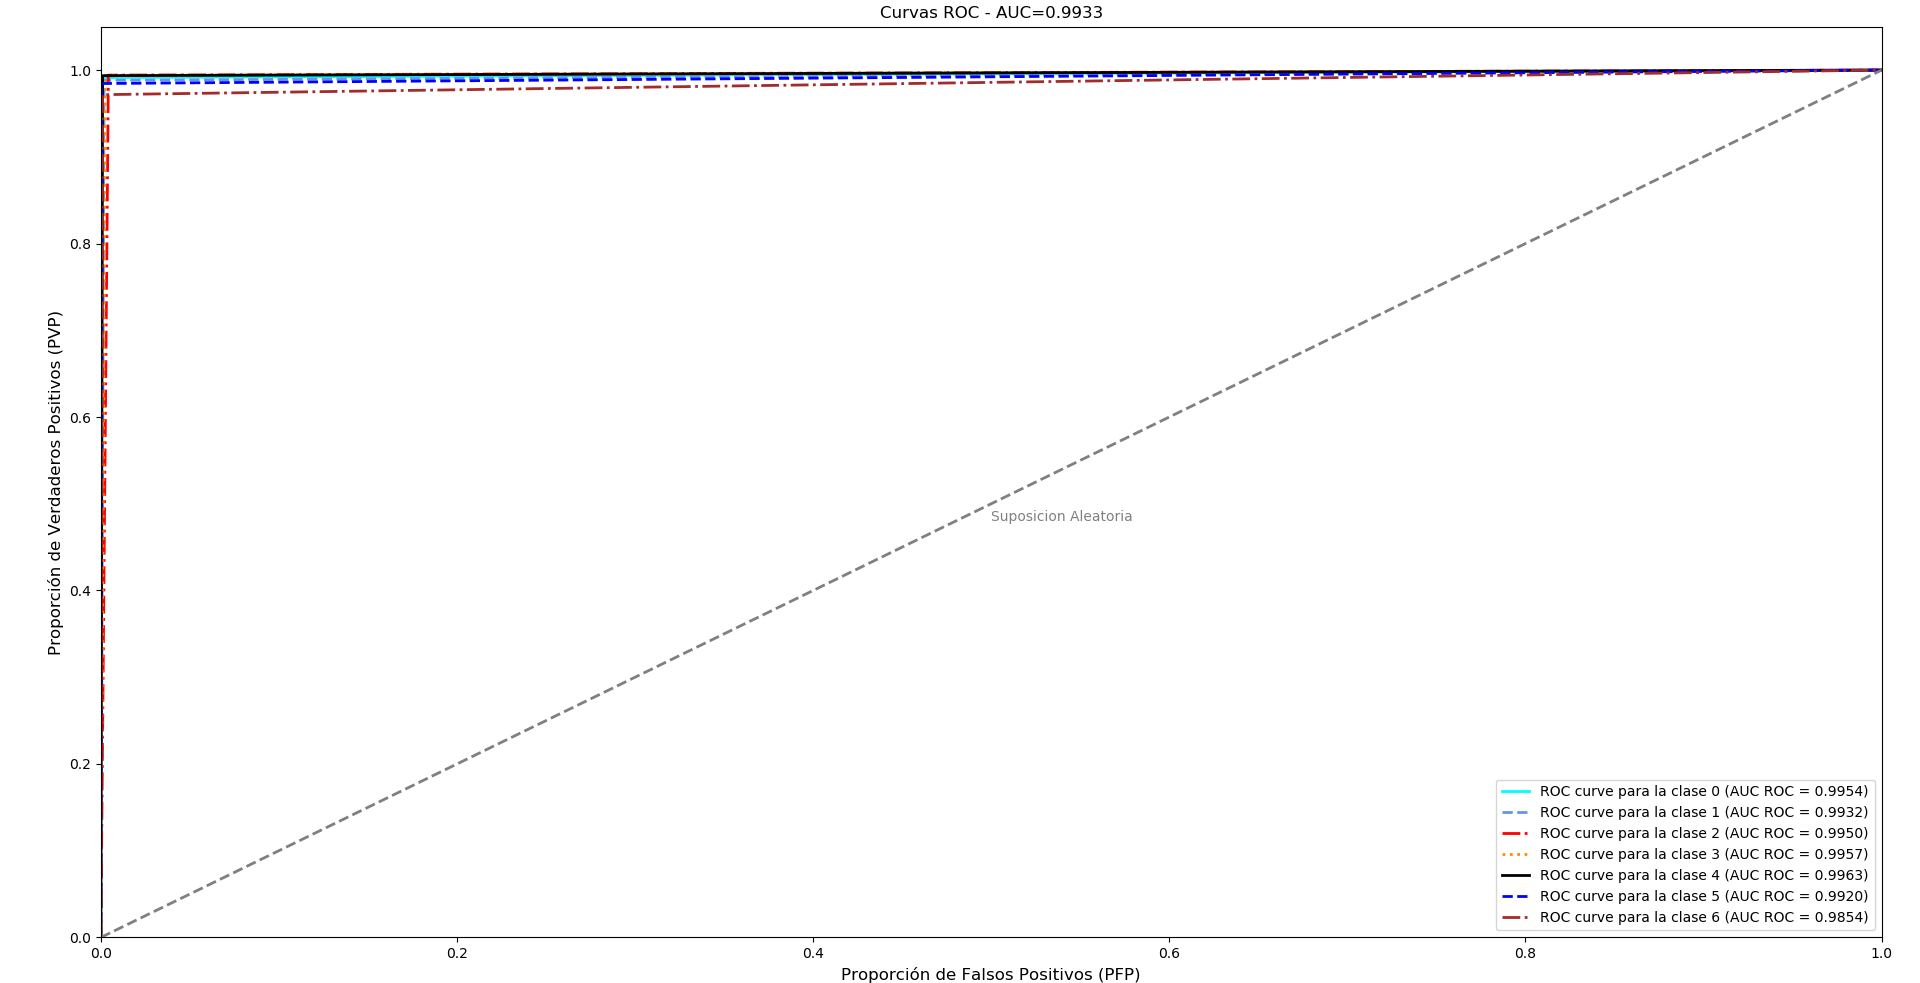
\includegraphics[width=1\textwidth, height=7.5cm]{images/desarrollo/testResults/peru/ROC_curve_modelE} 
						%\end{center}
						\begin{center}
						\caption{\small{Área debajo de la Curva ROC del Modelo E - Dataset de imágenes de Perú}}
						
						{\small{\fontsize{10}{16.8}\selectfont {Fuente: Elaboración propia}}}
						\end{center}
						\vspace{-1.5em}
					\end{figure}
		%------------------------------------------------------------------------------------------------------------------------------------------------------------
		\subsection{Curvas PR - AUC}  
					\begin{figure}[H]
						%\begin{center}
						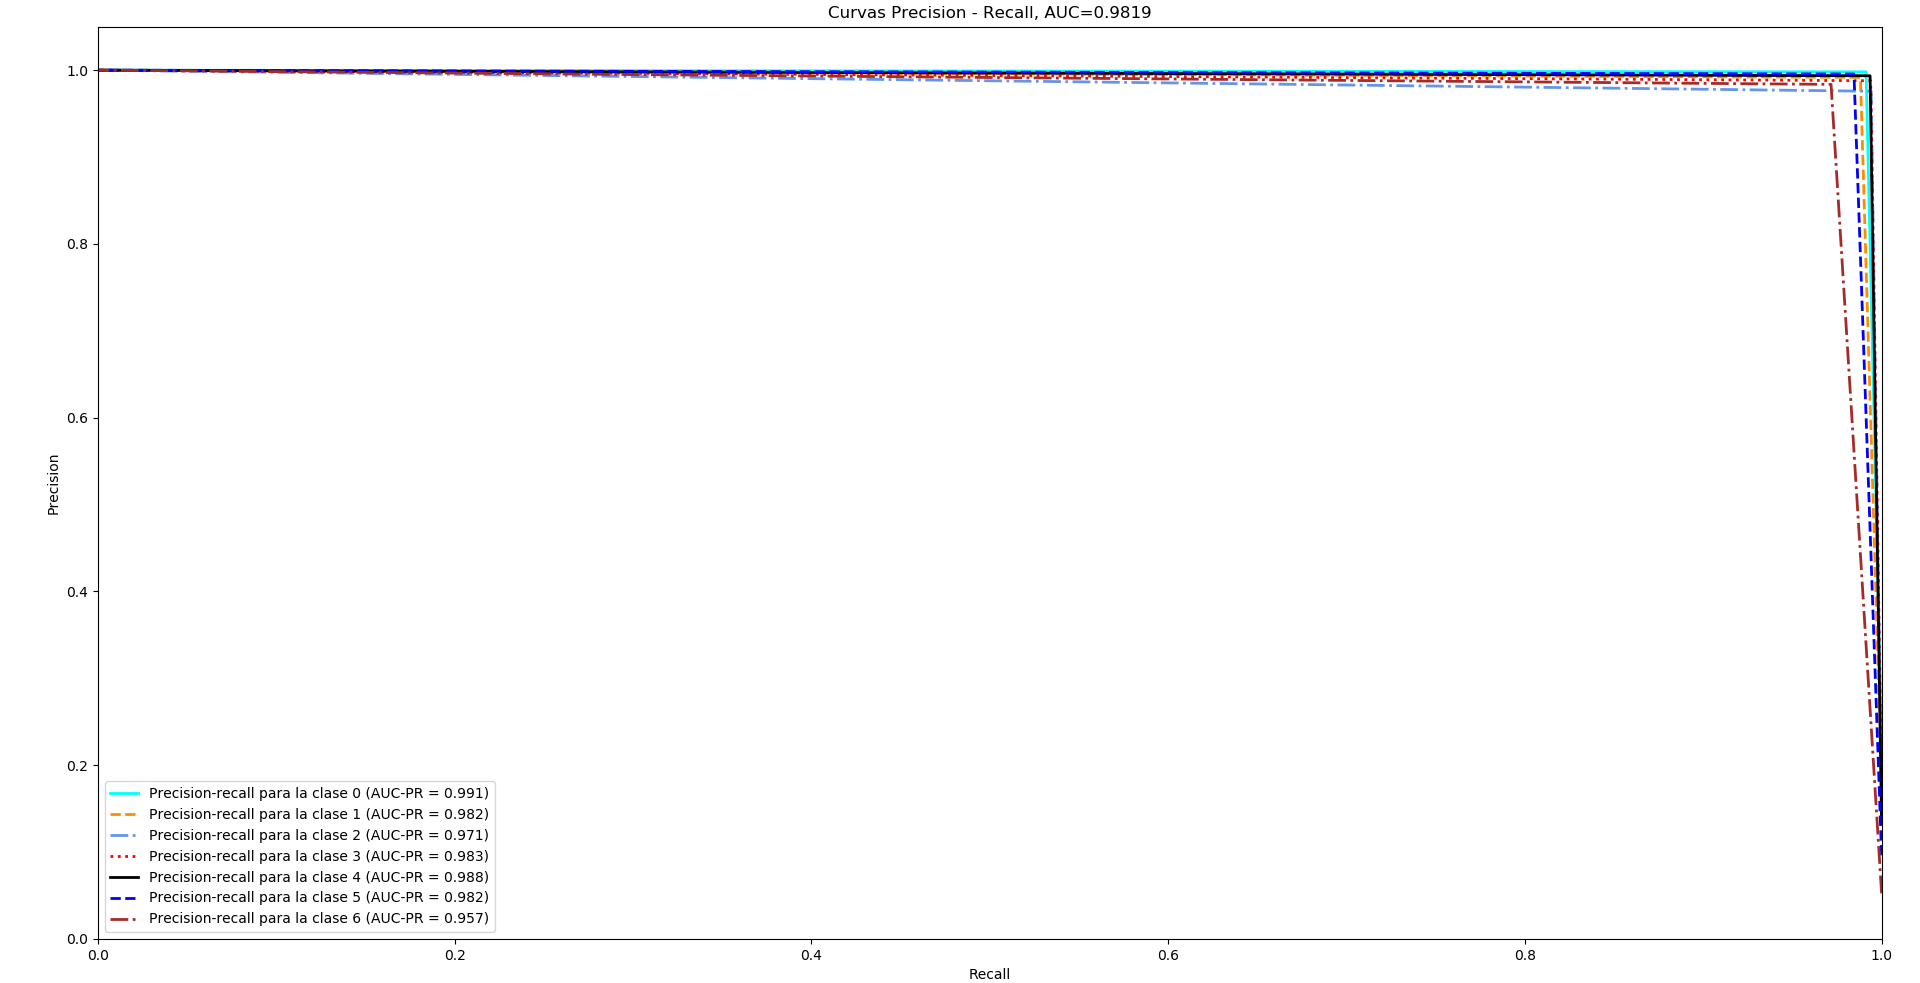
\includegraphics[width=1\textwidth, height=7.5cm]{images/desarrollo/testResults/peru/PR_curve_modelE} 
						%\end{center}
						\begin{center}
						\caption{\small{Área debajo de la Curva PR del Modelo E - Dataset de imágenes de Perú}}
						{\small{\fontsize{10}{16.8}\selectfont {Fuente: Elaboración propia}}}
						\end{center}
						\vspace{-1.5em}
					\end{figure}
	\newpage
	
	
		
	\section{Reconocimiento de Señal}
		Para continuar con la evaluación del rendimiento en el reconocimiento de señales de tránsito, los modelos para el Dataset de señales de Alemania y Perú con mejores resultados fueron utilizados en un aplicación programada en lenguaje python, la cual se encarga de analizar y reconocer una nueva imagen que contenga una señal de tránsito.

		A continuación se muestran los pasos necesarios para reconocer una imagen que contiene una señal de tránsito:

		\begin{figure}[H]
			\begin{center}
			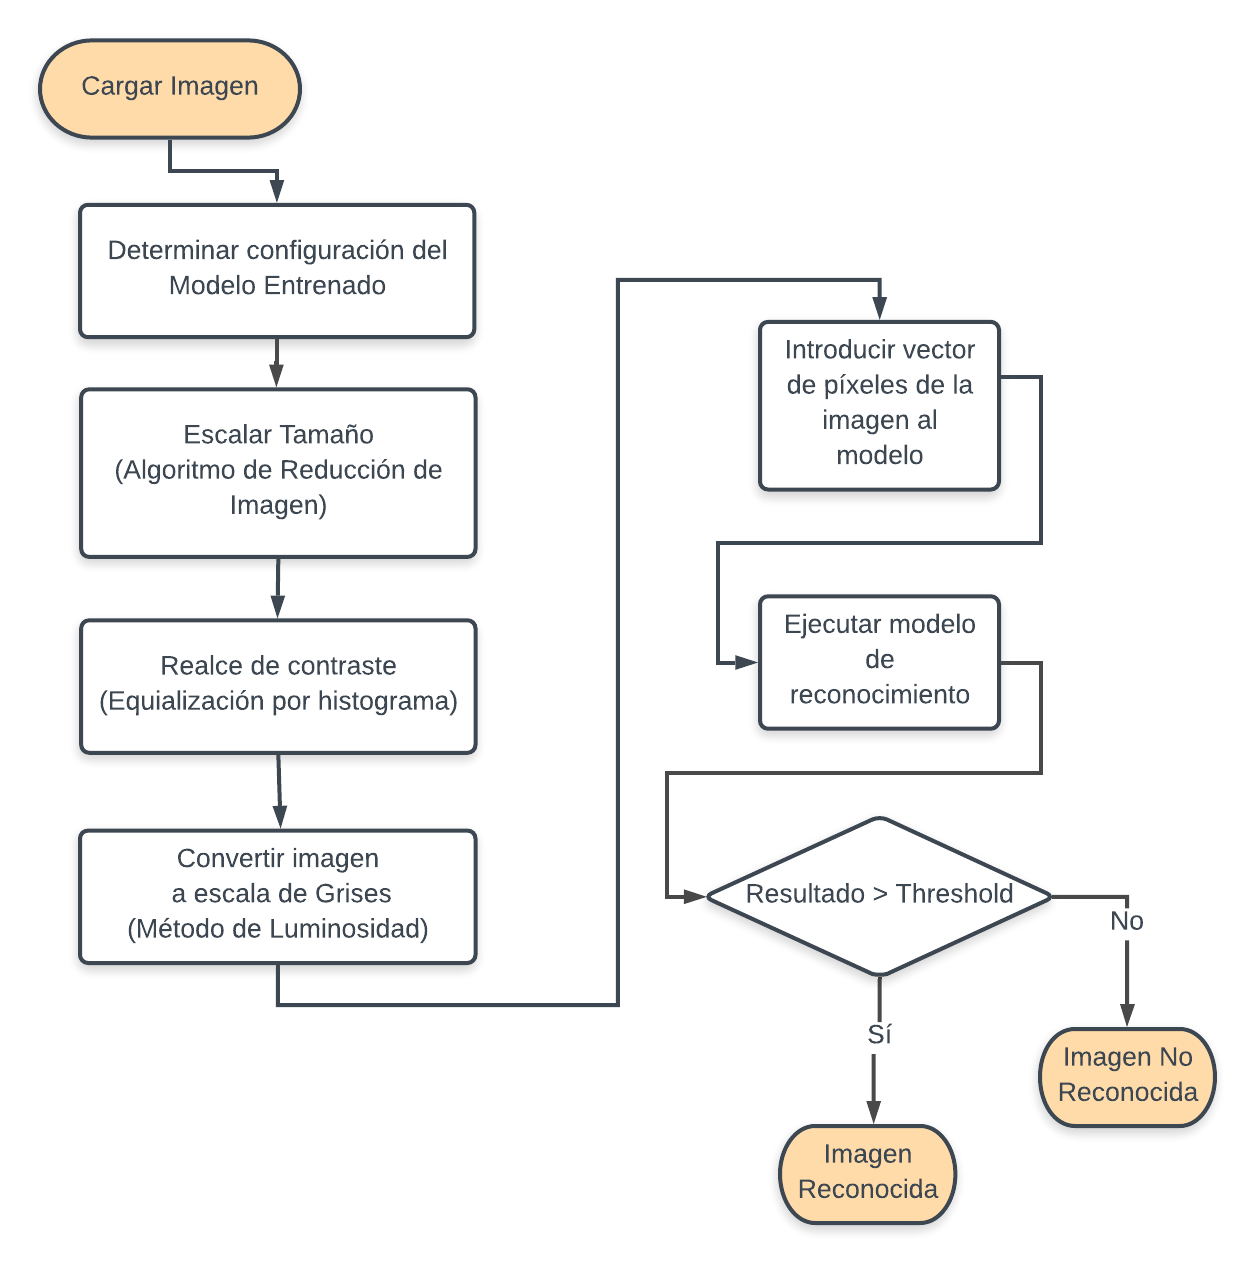
\includegraphics[width=0.8\textwidth,  height=10cm]{images/reconyzeFLow} 
			\end{center}
			\begin{center}
			\vspace{1em}
			\caption{\small{Flujograma para el reconocimiento de una señal de tránsito}}
			{\small{\fontsize{10}{16.8}\selectfont {Fuente: Elaboración propia}}}
			\end{center}
			\vspace{-1.5em}
		\end{figure}


	
		\subsection{Interfaz de Aplicación}
			\begin{figure}[H]
				%\begin{center}
				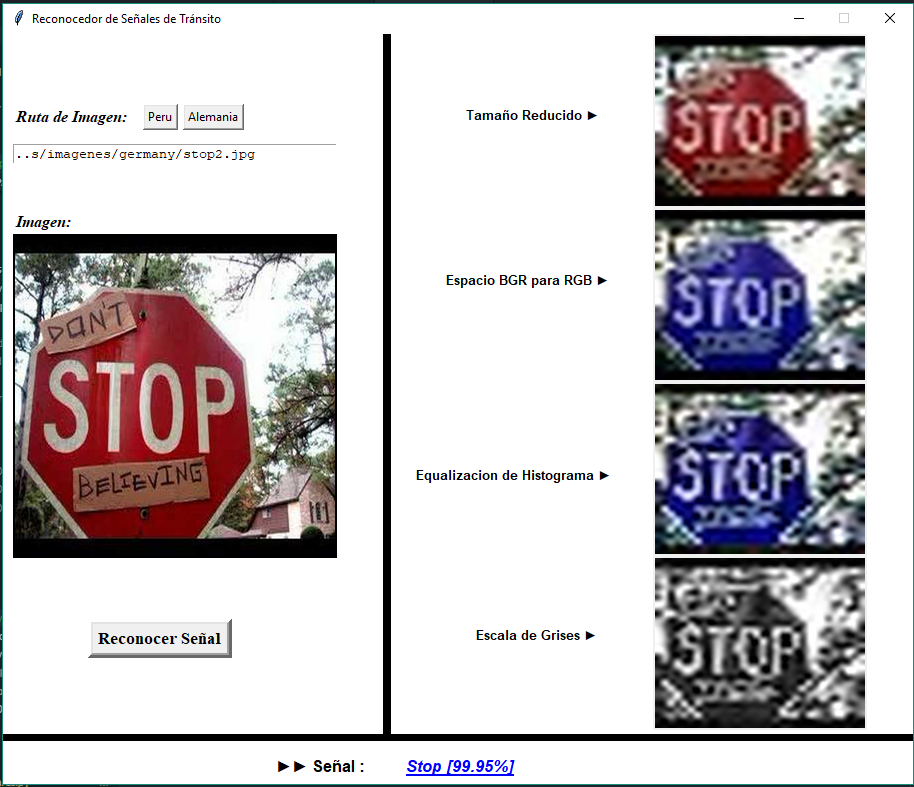
\includegraphics[width=1\textwidth,  height=12cm]{images/interfazWithGermSign} 
				%\end{center}
				\begin{center}
				\vspace{1em}
				\caption{\small{Interfaz reconociendo Señal de Tránsito “Wild Animals Crossing” - Alemania}}
				{\small{\fontsize{10}{16.8}\selectfont {Fuente: Elaboración propia}}}
				\end{center}
				\vspace{-1.5em}
			\end{figure}

			\begin{figure}[H]
				%\begin{center}
				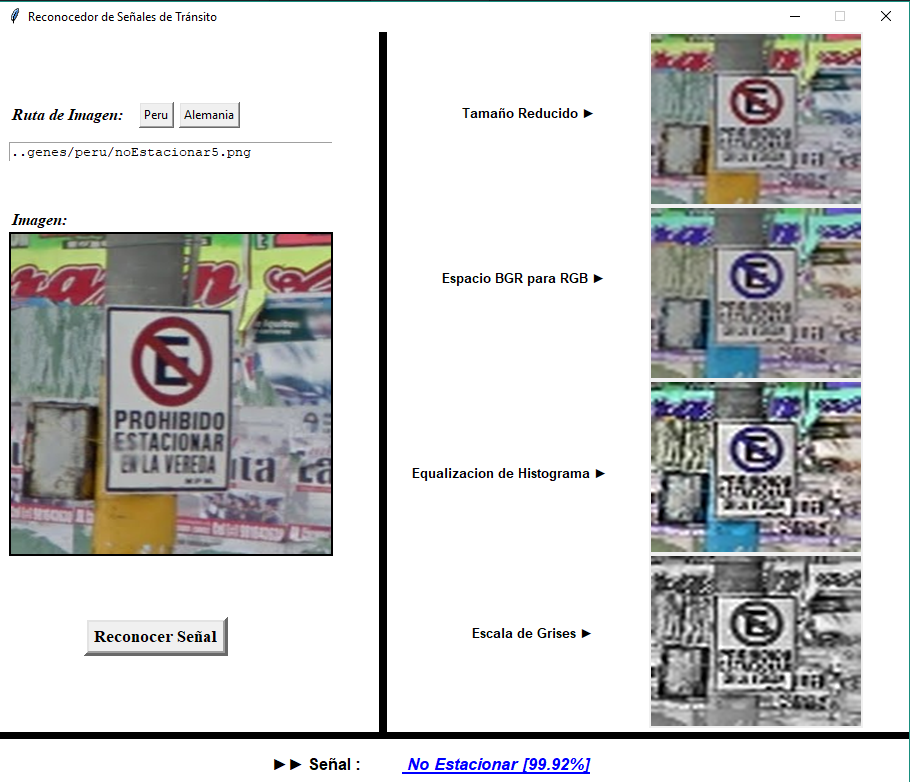
\includegraphics[width=1\textwidth, height=\textheight,keepaspectratio]{images/interfazWithPeruvSign} 
				%\end{center}
				\begin{center}
				\vspace{1.8em}
				\caption{\small{Interfaz reconociendo Señal de Tránsito “No Estacionar” - Perú}}
				{\small{\fontsize{10}{16.8}\selectfont {Fuente: Elaboración propia}}}
				\end{center}
				\vspace{-1.5em}
			\end{figure}